%% latex_185_norris_c.tex
%%
%% The following file is a skeleton file that demonstrates how to implement the IEEEtran.cls class
%% file in LaTeX. This file is intended for the CMPE185 Technical Writing for Engineers Course in 
%% which the students must write a tutorial aimed towards novice LaTeX users in the LaTex environment.
%%
%% This file is heavily adapted from Michael Shell's bare_adv.tex file made available at 
%% http://www.ieee.org/conferences_events/conferences/publishing/templates.html
%% ---------------------------------------------------------------------------------------------------

\documentclass[10pt,final,journal,compsoc]{IEEEtran}

%-----PACKAGES-------------------------------------------------------------------------------------

% Packages include extra commands that allow for additional formatting, ranging from Graphics, Math, to Alignment. The command to include packages will always look similar to \usepackage{} where the package name is within the curly brackets {}. Packages are defined in the preamble, i.e., between the \documentclass{} and \begin{document} commands.

% The following link takes you to a list of additional packages that may not be listed here. http://en.wikibooks.org/wiki/LaTeX/Package_Reference

% TO INCLUDE PACKAGES: 
% - Open the file ''latex_sample_packages.tex'' from the .zip folder.
% - From this file, COPY the code for the package you want to include and PASTE into your own .tex file.
% - Uncomment the package you want to include and load, i.e., remove the ''%'' in front of the \usepackage{package_name}.
 

% Copy package text here:

\usepackage{listings}
\usepackage{tikz}
\usepackage{pgfplots}
\usepackage{xfrac}
\usepackage{amsmath}

\lstset{
  language=TeX,
  aboveskip=3mm,
  belowskip=3mm,
  showstringspaces=false,
  columns=flexible,
  basicstyle={\small\ttfamily},
  numbers=none,
  breaklines=true,
  breakatwhitespace=true,
  tabsize=3,
  keywords={documentclass, begin},
}

% This is an example of how a \usepackage{} command should be included. You will need to include more packages to complete this assignment.



% ----------------------------------
% -    The DOCUMENT Environment    -
% ----------------------------------

\begin{document}

% The following commands are self explanatory. Insert your title, author and date into each command's curly bracket. You can include the abstract, paper header and paper footer information in this section then conclude the section with the command \maketitle (shown as the last line at the end of this section).

\title{How to Create Your First Document in \LaTeX}
\author{By Christian Norris}
\date{\today}

% The paper headers
% Note: the only time the second header will appear is for the odd numbered pages
% after the title page when using the twoside option.
\markboth{\LaTeX\ IEEE Template Tutorial}
{Norris \MakeLowercase{\textit{et al.}}: CSE 185}

% The publisher's ID mark
\IEEEpubid{0000--0000/00\$00.00~\copyright~2007 IEEE}


% for Computer Society papers, we must declare the abstract and index terms
% PRIOR to the title within the \IEEEcompsoctitleabstractindextext IEEEtran
% command as these need to go into the title area created by \maketitle.
\IEEEcompsoctitleabstractindextext{%
\begin{abstract}
%\boldmath
\LaTeX\ is a free markup language for creating highly customizable documents. This paper will walk the reader through the steps of creating their first document in LaTeX, as well as showing them some basic commands to get started in personalizing their project.
\end{abstract}

% Note that keywords are not normally used for peerreview papers.
\begin{IEEEkeywords}
CMPE185, \LaTeX\ Tutorial, IEEEtran, journal, \LaTeX, paper, template.
\end{IEEEkeywords}}

\maketitle


% ---------------------------------
% -    The SECTION Environment    -
% ---------------------------------

\tableofcontents

% -------------------------------
% --         SECTION 1         --
% -------------------------------

\section{Introduction}

\IEEEPARstart{H}{ave} you heard of \LaTeX\ before, but have no idea how to create your own document or even where to start? Don't worry---its much easier than you think! In this paper, I will teach you how to create your first document in \LaTeX, as well as some basic features so that you can start to personalize your document and show the world your ideas!
\subsection{Why \LaTeX?}
\LaTeX\ is both easy to use and extremely powerful, making it the most popular way to create personalized documents in most industries. Whether you are a professional or a student, creating your documentation in \LaTeX\ will show the world that you not only know what you are doing, but that you can do it in style.

% needed in second column of first page if using \IEEEpubid:
%\IEEEpubidadjcol

\subsection{Why this tutorial?}
I created this tutorial with new users specifically in mind, with the goal of making \LaTeX\ less intimidating. Here you will find much of the basic information you will need to get you up and running so you can start creating the documentation of your dreams.



% -------------------------------
% --         SECTION 2         --
% -------------------------------

\section{Getting Started}
Here I will show you some very simple things you will need to know when creating your first \LaTeX\ document.

\subsection{Environments}
\textit{Environments} are a way to tell \LaTeX\ to format a section of your document in a special way. They are comprised of two tags: \verb|\begin{}| and \verb|\end{}|, where everything between them is the environment. While defining environments can give you a lot of advanced flexibility, we won't be doing any of that in this tutorial. Instead, here is a simple example of an environment that centers text:

\begin{lstlisting}
\begin{center}
This text is centered in my document because it exists within this special environment!
\end{center}
\end{lstlisting}

And here's how it looks:
\begin{center}
This text is centered in my document because it exists within this special environment!
\end{center}

\subsection{Creating your document's environment}
All \LaTeX\ documents must be contained within an environment that will describe the overarching style of the entire project. This is created using the \verb|\documentclass{}| keyword, and can be customized to your heart's content.

After defining your document class, you can then create the environment that will contain your entire paper with the \verb|\begin{document}| and \verb|\end{document}| commands.

Here's an example of creating a very basic document class:

\begin{lstlisting}
\documentclass{article}

\begin{document}
Hello World!
\end{document}
\end{lstlisting}

\subsection{Importing packages}
Creating super advanced custom styles for \LaTeX\ can be tiresome, and why re-invent the wheel if you don't need to? To support this, \LaTeX\ has a neat feature called \textit{packages} that allows you to import more complex ways of formatting your document. We'll go through some examples of packages later, but for now just remember that you can import a package with the keyword \verb|\usepackage{<package_name>}| placed {\bf before} your \verb|\begin{document}|.

\subsection{Title and heading information}
Generally speaking, you will want to start your document off with the title, author, and date. These all have their own dedicated commands (\verb|\title{}|, \verb|\author{}|, and \verb|\date{}| respectively) and should be placed at the top of your document directly under \verb|\begin{document}|.

After this, you can use the \verb|\maketitle| command to tell \LaTeX\ to handle your heading information. Depending on your document class, \LaTeX\ will either place it at the top of your first page or create a separate title page. That being said, if you are using the \textit{article} document class (which was shown in the above example), then it will place the heading information at the top of your first page.

Here is an example of what that would look like all together:
\begin{lstlisting}
\title{My First LaTeX Document}
\author{By Christian Norris}
\date{\today}
\maketitle
\end{lstlisting}

Note: \LaTeX\ can calculate the current date for you with \verb|\today| so you don't have to type it out yourself. What a helpful feature!

\subsection{Reserved characters}
One last thing to know before creating your first document is that \LaTeX\ has some \textit{reserved characters}. These are used to tell \LaTeX\ that you want to do something special, whether that's formatting, using a keyword, etc. Here is a list of the reserved characters:

\verb|# $ % & { } _ ~ ^ \|

Here is what each of these reserved characters do:
\begin{itemize}
  \item \# designates the parameters for macro commands
  \item \$ is used to enter math mode
  \item \% creates inline comments
  \item \& ensures spacing around operators such as =, \textless, and \textgreater
  \item \{ and \} are used to designate command arguments
  \item \_ signifies a subscript in math mode
  \item \~{} forces a non-breaking space between text
  \item \^{} signifies a superscript in math mode
  \item \textbackslash\ signifies to \LaTeX that we are using a command
  \item \textbackslash \textbackslash\ destroys paragraph formatting
\end{itemize}

In order to use most of these in your document's in the text body, simply put a backslash \textbackslash in front of the character. However to print the last three in the list, you will have to handle these slightly \\ differently. To get a tilde (\~{}) you can use \verb|\~{}|, for a caret (\^{}) use \verb|\^{}|, and for a backslash use the command \verb|\textbackslash|.



% -------------------------------
% --         SECTION 3         --
% -------------------------------

\section{Formatting and Organization}
Now that you know how to set up your document, you can learn how to \textit{format} and \textit{organize}.

\subsection{Sections}
As you probably have noticed, this tutorial is broken up into sections. This is a super easy way to organize your document, and is very intuitive for the reader. To create a section, use the command \verb|\section{<header_text>}|. This will automatically number your section, and the text within the curly brackets will be the section header text. You can also create subsections and sub-subsections with the commands \verb|\subsection{<header_text>}| and \verb|\subsubsection{<header_text>}| respectively. You can then fill out the body text by simply writing underneath the section/subsection command.

\subsubsection{Table of contents}
\LaTeX\ has a tool to automatically create a table of contents from these sections that you create. While it is usually placed near to top of your document, you can place it anywhere you'd like with the \verb|\tableofcontents| command.

If you would like to omit a section from the table of contents, you can do this by simply adding an asterisk (*) before the header text like so: \verb|\section*{<header_text>}|

\subsection{Body text}
Any good written document will have body text within the sections and subsections. Creating this is super easy! All it you have to do is simply write normal text underneath the section header.

\subsubsection{Paragraphs}
You can create new paragraphs within your body text in multiple ways. The first (and simplest) way is to simply press your \textit{enter} key twice. having a blank line in between text will tell \LaTeX\ that you want to start a new paragraph. If you want to create a new paragraph without adding extra whitespace in your \LaTeX\ code, you can do so with the \verb|\par| command. Both of these will achieve the same effect, so you can decide to use whichever one you prefer.

\subsection{Text formatting}
\LaTeX\ provides you with a myriad of ways to format your text with simple inline commands. While there are tons of different formatting tools, here is a list of the basic ones that will definitely be enough to get you started:

\begin{itemize}
  \item \textbf{Bold}: \verb|\textbf{text}|
  \item \textit{Italics}: \verb|\textit{text}|
  \item \underline{Underline}: \verb|\underline{text}|
  \item \emph{Emphasis}: \verb|\emph{text}|
\end{itemize}

Multiple of these can be combined by nesting the commands within each other. An example of both \textbf{bold} and \underline{underlined} text would look like this: \verb|\textbf{\underline{Hello!}}|

The emphasis command also works in a special way---it will format your text differently depending on the type of formatting already applied to your text. \verb|\emph{}| will usually italicize the text, however it will un-italicize text that is already in italics.



% -------------------------------
% --         SECTION 4         --
% -------------------------------

\section{Common \LaTeX\ Document Additions}
In this section, I will teach you how to use a few of the most common features that \LaTeX\ has to make your document really shine. We will go over how to insert \textit{tables}, \textit{pictures}, \textit{titration plots}, and \textit{mathematical formulas}.

\subsection{Tables}
In \LaTeX, tables are highly customizable. Although it might seem a bit confusing at first, don't worry! It is a very intuitive system once it clicks.

\subsubsection{A very simple table}
Here is an example of a very simple table with no borders:

\begin{center}
\begin{tabular}{ c c c }
 cell1 & cell2 & cell3 \\ 
 cell4 & cell5 & cell6 \\  
 cell7 & cell8 & cell9 \\
\end{tabular}
\end{center}
\vspace{10px}

And here is what the \LaTeX\ code looks like:

\begin{lstlisting}
\begin{center}
\begin{tabular}{ c c c }
 cell1 & cell2 & cell3 \\ 
 cell4 & cell5 & cell6 \\  
 cell7 & cell8 & cell9 \\ 
\end{tabular}
\end{center}
\end{lstlisting}

The \verb|\begin{center}| block centers the table. While this isn't necessary, it is standard for tables to be centered. 

The \verb|\begin{tabular}| block is what creates the actual table. \verb|{ c c c }| tells \LaTeX\ that you want three columns to your table. In this field, 'c' is used to center the text in each cell, however you can also use 'l' and 'r' for left and right alignment respectively.

\verb|cell1 & cell2 & cell3 \\| is a single row is cells, where you can fill in the text for each cell separated by an '\&'. Each row should be finished off with a double backslash, which signifies to \LaTeX\ that the row is finished. Remember to make the number of cells in each row the same as the number of columns as specified above.

\subsubsection{Adding borders to a table}
Here is the same table we created above, except with borders this time:

\begin{center}
\begin{tabular}{ |c||c||c| } 
 \hline
 cell1 & cell2 & cell3 \\ 
 cell4 & cell5 & cell6 \\ 
 cell7 & cell8 & cell9 \\ 
 \hline
\end{tabular}
\end{center}
\vspace{10px}

And here is what the \LaTeX\ code looks like:

\begin{lstlisting}
\begin{center}
\begin{tabular}{ |c||c||c| } 
 \hline
 cell1 & cell2 & cell3 \\ 
 cell4 & cell5 & cell6 \\ 
 cell7 & cell8 & cell9 \\ 
 \hline
\end{tabular}
\end{center}
\end{lstlisting}

In this table, there are two main changes: \verb=|c||c||c|= and \verb|\hline|.

The vertical bars ( | ) in \verb=|c||c||c|= create vertical lines between/around the cells. On the outside of the table, there are two single vertical bars which outline the sides of the table. Inbetween the cells are double vertical bars, which create double lines separating the columns. You can use as many vertical bars as you'd like to create that many lines.

The \verb|\hline| command is what creates the horizontal lines in the table. In this example, we only have a horizontal line on the top and bottom, however you can place them between whichever rows you'd like, and to create multiple horizontal lines between two rows, much like we did with the columns.

\subsubsection{Slightly more advanced table}
Now we can combine everything we've learned to far to create a beautiful looking table:

\begin{center}
\begin{tabular}{||c l c r||} 
 \hline
 Index & Name & Status & Earnings/hr \\
 \hline\hline
 1 & John & Yes & 13.43 \\ 
 \hline
 2 & Mary & No & 8.91 \\
 \hline
 3 & Steve & No & 10.78 \\
 \hline
 4 & Jill & Yes & 14.09 \\
 \hline
 5 & Tim & No & 4.02 \\
 \hline
\end{tabular}
\end{center}
\vspace{10px}

And here is what the \LaTeX\ code looks like:

\begin{lstlisting}
\begin{center}
\begin{tabular}{||c l c r||} 
 \hline
 Index & Name & Status & Earnings/hr \\
 \hline\hline
 1 & John & Yes & 13.43 \\ 
 \hline
 2 & Mary & No & 8.91 \\
 \hline
 3 & Steve & No & 10.78 \\
 \hline
 4 & Jill & Yes & 14.09 \\
 \hline
 5 & Tim & No & 4.02 \\
 \hline
\end{tabular}
\end{center}
\end{lstlisting}

While this table looks much better, nothing is being done here that we haven't already learned. You can see the combination of column alignments being used, as well as the varied number of horizontal and vertical lines being used to both outline the table and separate a header row from the rest of the entries.

\subsection{Figures}
While there are many kinds of figures that \LaTeX\ allows you to create, I will show you two of the most common types: \textit{pictures} and \textit{titration plots}.

\subsubsection{Importing pictures}
Adding pictures to your document is super easy in \LaTeX. Here is an example of what a picture would look like in your document with basic formatting:

\begin{figure}[h]
\centering
\includegraphics[width=1.5in]{slug.pdf}
\caption{Sammy the Slug}
\label{fig_slug}
\end{figure}

And here is what the \LaTeX\ code looks like:

\begin{lstlisting}
\begin{figure}[h]
\centering
\includegraphics[width=1.5in]{slug.pdf}
\caption{Sammy the Slug}
\label{fig_slug}
\end{figure}
\end{lstlisting}

In order to create the \LaTeX\ figure that holds the image you must wrap it inside of a \verb|\begin{figure}| block. You might notice that there is also a \verb|[h]| at the end of that first begin, and that is to set the positioning of the figure in your document. The 'h' tells \LaTeX\ to place the image at about the same place it appears in the source text. Some other options you can use instead of this are 't' to place at the top of the current page, 'b' to place at the bottom, and 'p' to put on a special page for figures only.

Inside of the figure block we have the \verb|\centering| command, which centers the figure.

Next is the \verb|\includegraphics[width]{<file_name>}| command. Inside of the square brackets you can specify the width or height of the image. Inside of the curly brackets is where you specify the file name/path to be displayed. PNG, JPG, and PDF are all supported file types.

Then we have the \verb|\caption{<caption>}| command where you can create a caption for your image. \LaTeX\ will automatically number your figures for you, so you just need to worry about the name.

Finally is the \verb|\label{<label>}| command which assigns a label name to your figure. This won't directly show in your document, however the label will allow us to reference this figure later in our document. I will go into more detail on this in section 5.1.2 of this tutorial.


\subsubsection{Creating titration plots}
While creating plots in \LaTeX\ can be quite advanced, I will show you a very simple example using data that you can find attached in the titration\_plot.pdf.

Before creating the titration plot, you will need to import a couple of packages into your \LaTeX\ document. Add the commands \verb|\usepackage{tikz}| and \verb|\usepackage{pgfplots}| at the top of your document before the \verb|\begin{document}| command. After that, you are ready to create!

Here is the example of a simple titration plot:

\begin{figure}[h]
\centering
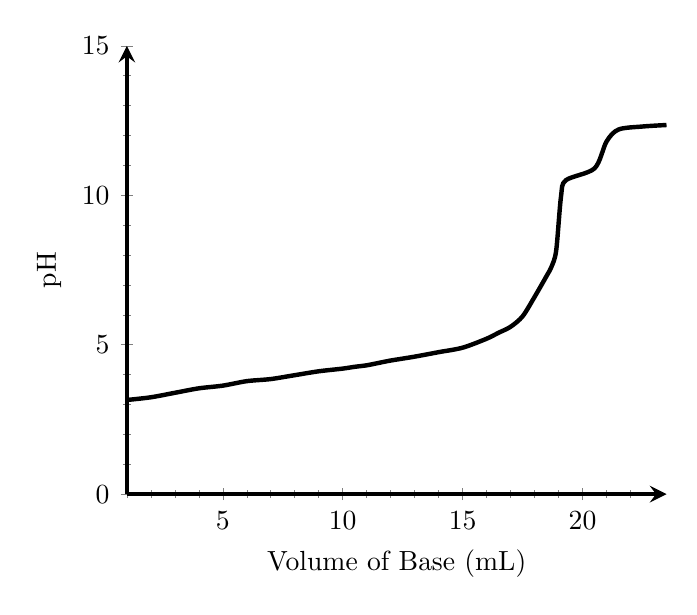
\begin{tikzpicture}
\begin{axis}[ axis x line=bottom, axis y line=left, minor tick num=4, ymin=0, ymax=15, ultra thick, xlabel={Volume of Base (mL)}, ylabel={pH} ]
\addplot[smooth] coordinates {
(1.0,3.15)(2.0,3.24)(3.0,3.39)(4.0,3.54)(5.0,3.63)(6.0,3.78)(7.0,3.85)(8.0,3.98)(9.0,4.11)(10.0,4.20)(10.5,4.26)(11.0,4.31)(11.5,4.39)(12.0,4.47)(13.0,4.60)(14.0,4.75)(15.0,4.90)(16.0,5.20)(16.5,5.40)(17.0,5.60)(17.5,5.95)(18.0,6.60)(18.5,7.30)(18.7,7.60)(18.9,8.15)(19.1,9.95)(19.3,10.50)(20.5,10.90)(21.0,11.80)(21.5,12.20)(22.5,12.30)(23.5,12.35)
};
\end{axis}
\end{tikzpicture}
\caption{pH levels of an unknown weak acid with a strong base (NaOH)}
\label{tit_plot}
\end{figure}

And here is what the \LaTeX\ code looks like:

\begin{lstlisting}
\begin{figure}[h]
\centering
\begin{tikzpicture}
\begin{axis}[ axis x line=bottom, axis y line=left, minor tick num=4, ymin=0, ymax=15, ultra thick, xlabel={Volume of Base (mL)}, ylabel={pH} ]
\addplot[smooth] coordinates {
(1.0,3.15) (2.0,3.24) (3.0,3.39)...
};
\end{axis}
\end{tikzpicture}
\caption{pH levels of an unknown weak acid with a strong base (NaOH)}
\label{tit_plot}
\end{figure}
\end{lstlisting}

There are three new commands in this code that are being used. If you would like to know what \verb|\begin{figure}|, \verb|\centering|, \verb|\caption{<caption>}|, and \verb|\label{<label>}| do, please check out the previous subsection on inserting pictures.

First, a \verb|\begin{tikzpicture}| is used to create the titration plot itself.

Next is \verb|\begin{axis}|, which creates the axes for the plot. Directly after this, you can use some rules to specify some of the specific behavior of the plots. Here we set the sides that the axes rest on, the minor tick intervals, axis ranges, axis thickness, and axis labels.

Finally is the \verb|\addplot| command. This is immediately followed by square brackets where you can specify some settings with predefined keywords. However for this example, we are just going to use \textit{smooth} to tell \LaTeX\ to smoothen the curve. After this are the curly brackets, which is normally used to specify an equation to plot. We can instead override this with the \textit{coordinates} keyword, and specify whatever coordinates we want to plot instead. While I only show a few of the points, you can view the rest of them on the titration\_plot.pdf


\subsection{Mathematical formulas}
One of the biggest things that \LaTeX\ is used for is creating beautiful mathematical equations without much effort. We are provided a ton of tools for doing so, and adding complex math to your document is both easy and intuitive.

\subsubsection{Equation environments}
First thing to note is that there are two ways to include mathematical equations into your document: inline and display.

Inline is just that---the equation will be shown in the current line without breaking the paragraph. This is great for single variables or shorter equations that you insert within text. Here is an example of an inline equation: \(5x^2 + 15 = 0\). To do this, simply wrap your equation inside of a \verb|\(| and \verb|\)|. In your \LaTeX\ code, the above example would look like this: \verb|\(5x^2 + 15 = 0\)|.

Display mode will break the current paragraph to show your equations. This is perfect for a series of equations or a longer proof where you need multiple lines back-to-back. You can create an equation in display mode in the same way is you would with in inline equation, except you use square brackets instead of parenthesis. Here is an example of an equation in display mode:

\[
a_0 + \frac{1}{a_1 +
        \frac{1}{a_2 +
          \frac{1}{\ddots}}} 
\]

\textit{Note:} some \LaTeX\ documents with use \$ and \$\$ to delimit inline and display equations respectively, however this is the standard for TeX, and \LaTeX\ does not officially support this syntax.

\subsubsection{Symbols}
\LaTeX\ gives us a wide variety of mathematical symbols, operators, and letters that we can use to create both simple and complex mathematical formulas. Here I will list some of the basic ones that should service what you need to do.

\begin{itemize}
  \item Greek Letters:
      \begin{itemize} 
        \item \(\alpha\) : \verb|\alpha|
        \item \(\beta\) : \verb|\beta|
        \item \(\delta\) : \verb|\delta|
        \item The uppercase version of \textit{some} letters can be used by capitalizing the first          letter of the command like so. \(\Delta\) : \verb|\Delta|
      \end{itemize}
  \item Delimiters:
      \begin{itemize} 
        \item \(\langle\) and \(\rangle\) : \verb|\langle| and \verb|\rangle|
        \item \(\{\) and \(\}\) : \verb|\{| and \verb|\}|
      \end{itemize}
  \item Common Functions:
      \begin{itemize} 
        \item \(\sqrt{abc}\) : \verb|\sqrt{abc}|
        \item \(\sqrt[n]{abc}\) : \verb|\sqrt[n]{abc}|
        \item \(\sum\) : \verb|\sum|
        \item \(\int\) : \verb|\int|
        \item \(\cos\) : \verb|\cos|
        \item \(\arccos\) : \verb|\arccos|
        \item \(\cosh\) : \verb|\cosh|
      \end{itemize}
  \item Misc. Symbols:
      \begin{itemize} 
        \item \(\infty\) : \verb|\infty|
        \item \(\cdot\) : \verb|\cdot|
        \item \(\ldots\) : \verb|\ldots|
        \item \(\vdots\) : \verb|\vdots|
        \item \(\ddots\) : \verb|\ddots|
        \item \(\forall\) : \verb|\forall|
        \item \(\exists\) : \verb|\exists|
        \item \(\prime\) : \verb|\prime|
        \item \(\surd\) : \verb|\surd|
      \end{itemize}
\end{itemize}

\subsubsection{Fractions}
To create fractions in \LaTeX\, you must use the \verb|\frac{a}{b}| command. The numerator is defined in the first set of curly brackets, and the denominator in the second set. Here is how that fraction would look in math mode: \(\frac{a}{b}\).

If you would like to use slanted fractions, you can import the \textit{xfrac} package with \verb|\usepackage{xfrac}| at the top of your document before the \verb|\begin{document}| command. This will give you access to \verb|\sfrac{1}{2}|, allowing for easier-to-read inline fractions that look like this: \sfrac{1}{2}

\subsubsection{Matrices}
Unfortunately, native \LaTeX\ doesn't have tools to create matrices. However, the \textit{amsmath} package provides us with simple tools for creating matrices. You can import this with \verb|\usepackage{amsmath}| at the top of your document before the \verb|\begin{document}| command. Here is an example of a very basic matrix:

\[
 \begin{matrix}
  a & b & c \\
  d & e & f \\
  g & h & i \\
 \end{matrix}
\]

And here is what the \LaTeX\ code looks like:

\begin{lstlisting}
\[
 \begin{matrix}
  a & b & c \\
  d & e & f \\
  g & h & i \\
 \end{matrix}
\]
\end{lstlisting}

In our code, each row is differentiated by two backslashes, and each cell within the rows are separated by an \&.

There is also another thing to note, and that is the \textit{matrix} keyword. This will create a blank matrix, however we can use other keywords to create different types of matrices. Here are a few of them:

\begin{itemize}
  \item \verb|pmatrix|: parenthesis (round brackets)
  \item \verb|bmatrix|: square brackets
  \item \verb|Bmatrix|: curly brackets
  \item \verb|vmatrix|: pipes
  \item \verb|Vmatrix|: double pipes
\end{itemize}

\subsubsection{Nesting functions}
Mathematical functions in \LaTeX\ can also be nested to create more complex equations. While these nests can get pretty deep and complicated, here is a simple example so you get the idea of how it is done:

\[
 \sqrt{ \frac{\pi}{2} }
\]

And here is what the \LaTeX\ code looks like:

\begin{lstlisting}
\[
 \sqrt{ \frac{\pi}{2} }
\]
\end{lstlisting}

\subsubsection{Superscripts and subscripts}
In many equations, superscripts and subscripts are vital in conveying the information needed. Luckily, these are super easy to implement in \LaTeX. For superscripts, the caret (\^) is used, and for subscripts, the underline (\_) is used. For example, creating \(x^2\) would be done by writing \verb|x^2|.

If you would like to add more to your superscript/subscript than just a single character, you need to put it in a block of curly brackets. For example, \verb|x^x+2| creates \(x^x+2\), however if we wanted to write \(x^{x+2}\), then we would need to surround our superscript with curly brackets like so: \verb|x^{x+2}|. This rule also applies to subscripts as well.

You can also apply superscripts and subscripts to most functions and symbols too! While there are tons of uses for this, here is an example of how we would use them to add parameters to a summation:

\[
\sum_{i=0}^n 
 \frac{i \cdot \pi}{2}
\]

And here is what the \LaTeX\ code looks like:

\begin{lstlisting}
\[
\sum_{i=0}^n 
 \frac{i \cdot \pi}{2}
\]
\end{lstlisting}



% -------------------------------
% --         SECTION 5         --
% -------------------------------

\section{Finishing Up Your Document}
All professional \LaTeX\ documents will wrap up with dedicated sections for \textit{appendices}, \textit{acknowledgements}, and \textit{references}. These are sections that allow you to properly cite and give credit to the sources that you pulled from for your document.

\subsection{Appendices}
In \LaTeX, we are provided with the \verb|\appendices| command which tells \LaTeX\ that all upcoming sections are appendices. These are sections that will still automatically be added to the table of contents, but will not have a section number associated with them. Here is an example of how to use the \verb|appendices| command in your code:

\begin{lstlisting}
\appendices

\section{}
Appendix one text goes here.

\section{Appendix title}
Appendix two text goes here.
\end{lstlisting}

In this example, we create two appendices. \LaTeX\ automatically titles these appendices "Appendix A" and "Appendix B" respectively. You might notice however that we specify a specific section title for our second appendix, which changes its title to "Appendix B: Appendix title".


\subsection{Acknowledgements}
Creating an acknowledgements section is fairly simple. This is simply a section where you can freely thank and give credit to anyone who helped you finish your document. The only major thing to note is that usually acknowledgement sections aren't included in the table of contents. To still create this section while also following this rule, refer to section 3.1.1 to learn how to omit a section from the table of contents.


\subsection{References}
The reference section is where you can directly cite the sources you used throughout your document. \LaTeX\ gives us great bibliography tools to allow us to easy declare sources and reference them within our text.

\subsubsection{Creating a bibliography}
To create a bibliography, we have to first declare a bibliography environment. Here is an example of the \LaTeX\ code to create a bibliography with a single entry:

\begin{lstlisting}
\begin{thebibliography}{1}
\bibitem{HKopka} Kopka, H., Daly P.W., \emph{A Guide to LaTeX}, Addison-Wesley, Reading, MA, 1999.
\end{thebibliography}
\end{lstlisting}

The \verb|\begin{thebibliography}{1}| command begins the bibliography section. The number in the curly brackets is the maximum number of entries that our bibliography can hold, which in our case we're just leaving it at one.

The \verb|\bibitem{HKopka}| command adds an entry into our bibliography. Inside the curly brackets is the citation key that you can use in your document to create in-text citations. Make sure to make the citation key both unique and descriptive to the specific citation.


\subsubsection{In-text citing}
So how do you create in-text citations? Well luckily, \LaTeX\ provides us with a simple command to do so: \verb|\cite{<citation_key>}|. Using this in your document will automatically add a number in brackets that references the position of the item in your bibliography. For example, if we were to write this in our \LaTeX\ code: \verb|... adding sections in LaTeX! \cite{HKopka}|, it would look like this in our document: "... adding sections in LaTeX! [1]".

\subsubsection{Referencing}
So now we know how to cite a source from our bibliography, but how do reference something that we created previously in our document? That is where referencing comes in. If you remember back to the end of section 4.2.1, we learned about the \verb|\label{<label>}| command. This applies a label to an object (in this case, a picture) that we can now refer to anywhere else in our document.

We do this by referencing the label name with the \verb|\ref{<label>}| command. Referencing an object with \verb|\ref| acts almost exactly like how \verb|\cite| does, however when shown in the final document, there are no brackets around the object's reference number. For example, if we were to write this in our \LaTeX\ code: \verb|... here is Figure \ref{fig_slug}.|, it would look like this in our document: "... here is Figure 1." \textit{Note}: fig\_slug is the figure that we created in section 4.2.1.




% -------------------------------
% --         SECTION 6         --
% -------------------------------

\section{Conclusion}
That just about wraps everything up! After reading this tutorial, you are now equipped with all of the tools to get started on your very own \LaTeX\ document! While all of the basics have already been covered, it is very possible that you will have questions or come across issues that are not covered in this tutorial. For that, I recommend searching the documentation over at www.overleaf.com/learn, as well as using your favorite search engine for any specific questions you might have.

In any case, glad you made it this far, and I wish you well on your journey creating your very own document in \LaTeX!

\appendices

\section*{Acknowledgements}
The main source I would like to thank in the development of this tutorial is Overleaf. Not only did they provide an excellent \LaTeX\ compiler for me to create this document on, but they also have tons of detailed, easy-to-read tutorials on how to use many of the functions and features displayed in this tutorial.

\begin{thebibliography}{1}
\bibitem{HKopka}
H.~Kopka and P.~W. Daly, \emph{A Guide to {\LaTeX}}, 3rd~ed.\hskip 1em plus
  0.5em minus 0.4em\relax Harlow, England: Addison-Wesley, 1999.
\end{thebibliography}


\end{document}
